\documentclass[aspectratio=169]{beamer}

\usetheme{Boadilla}
\usefonttheme{professionalfonts}
\setbeamertemplate{navigation symbols}{}
\setbeamertemplate{itemize items}[circle]
\setbeamertemplate{enumerate items}[default]
\setbeamertemplate{headline}{}

\usepackage[utf8]{inputenc}
\usepackage[T1]{fontenc}
\usepackage{lmodern}
\usepackage{amsmath}
\usepackage{booktabs}
\usepackage{tabularx}
\usepackage{array}
\usepackage{hyperref}
\usepackage[strings]{underscore}
\usepackage{listings}
\usepackage{tikz}
\usetikzlibrary{arrows.meta,positioning,fit,calc,shapes.geometric}
\usepackage{xcolor}

\definecolor{courseblue}{HTML}{12355B}
\definecolor{coursegold}{HTML}{C98A2E}
\definecolor{courseice}{HTML}{EEF3F8}
\definecolor{coursegreen}{HTML}{2F6B4F}
\definecolor{coursegray}{HTML}{4B5563}
\definecolor{codebg}{HTML}{F7F9FC}
\definecolor{codecomment}{HTML}{5E6C84}
\definecolor{codestring}{HTML}{0B6E4F}

\setbeamercolor{palette primary}{bg=courseblue,fg=white}
\setbeamercolor{palette secondary}{bg=coursegold,fg=white}
\setbeamercolor{palette tertiary}{bg=courseblue,fg=white}
\setbeamercolor{palette quaternary}{bg=coursegold,fg=white}
\setbeamercolor{structure}{fg=courseblue}
\setbeamercolor{frametitle}{bg=courseice,fg=courseblue}
\setbeamercolor{title}{fg=courseblue}
\setbeamercolor{block title}{bg=courseblue,fg=white}
\setbeamercolor{block body}{bg=courseice,fg=black}
\setbeamercolor{normal text}{fg=black,bg=white}
\setbeamercolor{alerted text}{fg=coursegold}

\setbeamerfont{footline}{size=\scriptsize}

\setbeamertemplate{footline}{
  \leavevmode
  \hbox{
    \begin{beamercolorbox}[wd=.33\paperwidth,ht=2.8ex,dp=1.2ex,leftskip=0.8em]{palette primary}%
      University of Trieste
    \end{beamercolorbox}%
    \begin{beamercolorbox}[wd=.49\paperwidth,ht=2.8ex,dp=1.2ex,center]{palette tertiary}%
      \coursename{} \textbar{} \coursecode
    \end{beamercolorbox}%
    \begin{beamercolorbox}[wd=.18\paperwidth,ht=2.8ex,dp=1.2ex,rightskip=0.8em plus1fil]{palette secondary}%
      \insertframenumber{} / \inserttotalframenumber
    \end{beamercolorbox}%
  }
}

\hypersetup{
  colorlinks=true,
  linkcolor=courseblue,
  urlcolor=coursegreen
}

\lstdefinestyle{coursepython}{
  language=Python,
  basicstyle=\ttfamily\footnotesize,
  keywordstyle=\color{courseblue}\bfseries,
  commentstyle=\color{codecomment}\itshape,
  stringstyle=\color{codestring},
  showstringspaces=false,
  columns=fullflexible,
  keepspaces=true,
  frame=single,
  framerule=0.6pt,
  rulecolor=\color{courseblue},
  backgroundcolor=\color{codebg},
  xleftmargin=0.4em,
  xrightmargin=0.4em,
  aboveskip=0.4em,
  belowskip=0.2em
}

\newcommand{\coursename}{Data-driven Systems Engineering}
\newcommand{\coursecode}{440MI / 305SM}
\newcommand{\coursefooter}{}

\newcommand{\learninggoals}[1]{
  \begin{block}{Learning goals}
  #1
  \end{block}
}

\newcommand{\repoactivity}[1]{
  \begin{block}{Repo activity}
  #1
  \end{block}
}

\newcommand{\readinglist}[1]{
  \begin{block}{Papers and materials}
  {\footnotesize #1}
  \end{block}
}

\newcommand{\coursecontextframe}[5]{
  \begin{frame}{Course Map and Running Cases}
  \centering
  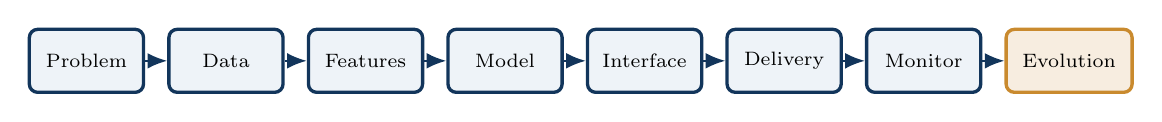
\begin{tikzpicture}[node distance=0.28cm]
  \node[flowbox, minimum width=1.45cm, minimum height=0.8cm] (problem) {\scriptsize Problem};
  \node[flowbox, minimum width=1.45cm, minimum height=0.8cm, right=of problem] (data) {\scriptsize Data};
  \node[flowbox, minimum width=1.45cm, minimum height=0.8cm, right=of data] (features) {\scriptsize Features};
  \node[flowbox, minimum width=1.45cm, minimum height=0.8cm, right=of features] (model) {\scriptsize Model};
  \node[flowbox, minimum width=1.45cm, minimum height=0.8cm, right=of model] (interface) {\scriptsize Interface};
  \node[flowbox, minimum width=1.45cm, minimum height=0.8cm, right=of interface] (delivery) {\scriptsize Delivery};
  \node[flowbox, minimum width=1.45cm, minimum height=0.8cm, right=of delivery] (monitor) {\scriptsize Monitor};
  \node[accentbox, minimum width=1.6cm, minimum height=0.8cm, right=of monitor] (evolution) {\scriptsize Evolution};
  \foreach \a/\b in {problem/data,data/features,features/model,model/interface,interface/delivery,delivery/monitor,monitor/evolution} {
    \draw[arrow] (\a) -- (\b);
  }
  \end{tikzpicture}

  \vspace{0.5em}
  \begin{block}{Today in the course}
  \textbf{Focus:} #1

  \textbf{Bridge:} #2
  \end{block}

  \begin{columns}[T]
  \column{0.48\textwidth}
  \begin{block}{Fraud case}
  {\footnotesize #3}
  \end{block}
  \column{0.48\textwidth}
  \begin{block}{Pasteurization case}
  {\footnotesize #4}
  \end{block}
  \end{columns}

  \vspace{0.3em}
  {\footnotesize \textbf{Course thread:} #5}
  \coursefooter
  \end{frame}
}

\newcommand{\classclosingframe}[4]{
  \begin{frame}{From This Class to the Next}
  \begin{block}{What stays with us}
  #1
  \end{block}

  \begin{columns}[T]
  \column{0.48\textwidth}
  \begin{block}{Project use}
  {\footnotesize #2}
  \end{block}
  \column{0.48\textwidth}
  \begin{block}{Next connection}
  {\footnotesize #3}
  \end{block}
  \end{columns}

  \vspace{0.3em}
  {\footnotesize \textbf{Course thread:} #4}
  \coursefooter
  \end{frame}
}

\tikzset{
  flowbox/.style={
    rounded corners=3pt,
    draw=courseblue,
    fill=courseice,
    very thick,
    minimum width=2.2cm,
    minimum height=0.9cm,
    align=center,
    font=\small
  },
  accentbox/.style={
    rounded corners=3pt,
    draw=coursegold,
    fill=coursegold!15,
    very thick,
    minimum width=2.2cm,
    minimum height=0.9cm,
    align=center,
    font=\small
  },
  arrow/.style={
    -{Latex[length=2.5mm,width=2mm]},
    thick,
    draw=courseblue
  }
}


\title{Class 6: Files, pandas, and Plotting}
\author{\coursename}
\date{}

\begin{document}

\frame{\titlepage \coursefooter}

\begin{frame}{Agenda}
\begin{itemize}
\item File handling in Python: opening, reading, writing.
\item Why pandas exists: the DataFrame and Series structures.
\item Reading tabular data into a DataFrame.
\item Selecting data with \texttt{loc}, \texttt{iloc}, and boolean masks.
\item A first look at plotting with pandas and Matplotlib.
\end{itemize}
\coursefooter
\end{frame}

\begin{frame}{Learning goals}
\learninggoals{
\begin{itemize}
\item Open a file in the correct mode for the task at hand.
\item Explain the difference between a pandas Series and a DataFrame.
\item Load a real dataset into a DataFrame with \texttt{pd.read\_csv}.
\item Select rows and columns with \texttt{loc}, \texttt{iloc}, and a boolean condition.
\item Produce a first plot directly from a DataFrame.
\end{itemize}
}
\coursefooter
\end{frame}

\coursecontextframe
{Getting data in and out of Python, and a first look at it visually.}
{Variables and loops manipulate values already in memory; this class is about where those values come from and how we glance at them.}
{The fraud model is trained from a CSV pulled straight into a DataFrame, and its artifacts are written and read back as pickle files on disk.}
{The pasteurization case writes and rereads sensor batches the same way, before any streaming or dashboard logic gets involved.}
{Nothing downstream --- EDA, modeling, serving --- can happen until data reliably gets in and out of the program.}

\begin{frame}{File handling in Python}
\begin{itemize}
\item \texttt{open(filename, mode)} is the core function for reading, writing, and appending files.
\item Always close what you open, or use \texttt{with open(...) as f:} so Python closes it automatically.
\end{itemize}
\begin{tabularx}{\textwidth}{>{\bfseries}l X}
Mode & Meaning \\
\toprule
\texttt{r} & Read (default); errors if the file does not exist. \\
\texttt{w} & Write; creates the file, overwrites if it exists. \\
\texttt{a} & Append; creates the file if needed, adds to the end otherwise. \\
\texttt{x} & Create; errors if the file already exists. \\
\texttt{t} / \texttt{b} & Text mode (default) or binary mode, e.g.\ for pickled objects. \\
\bottomrule
\end{tabularx}
\coursefooter
\end{frame}

\begin{frame}[fragile]{Writing a file, for real}
\begin{lstlisting}[style=coursepython]
with open('model.pkl', 'wb') as f:
    pickle.dump(cls, f)

with open('scaler.pkl', 'wb') as f:
    pickle.dump(scaler, f)
\end{lstlisting}
\begin{itemize}
\item From `streamlit/modeling.py`: mode \texttt{'wb'} combines write and binary, because a pickled Python object is not text.
\item The trained model and scaler exist on disk only because of these two \texttt{open()} calls.
\end{itemize}
\coursefooter
\end{frame}

\begin{frame}[fragile]{Reading it back}
\begin{lstlisting}[style=coursepython]
model = pickle.load(open('model.pkl', 'rb'))
scaler = pickle.load(open('scaler.pkl', 'rb'))
\end{lstlisting}
\begin{itemize}
\item `App_Credit_Card.py` reopens the same two files in \texttt{'rb'} mode --- read, binary.
\item Whoever writes a file and whoever reads it must agree on the mode; mixing text and binary modes is a common source of errors.
\end{itemize}
\coursefooter
\end{frame}

\begin{frame}{Why pandas}
\begin{itemize}
\item pandas is a fast, flexible library for tabular data analysis; many ML libraries accept its structures directly as input.
\item \textbf{Series}: a single labeled column of data.
\item \textbf{DataFrame}: a table made of one or more Series sharing a row index, similar to a spreadsheet or a relational table.
\item pandas is column-oriented: operations on a whole column are typically fast and expressive.
\end{itemize}
\coursefooter
\end{frame}

\begin{frame}[fragile]{Reading tabular data into a DataFrame}
\begin{lstlisting}[style=coursepython]
import pandas as pd

url = 'https://storage.googleapis.com/download.tensorflow.org/data/creditcard.csv'
df = pd.read_csv(url)
\end{lstlisting}
\begin{itemize}
\item This is the exact loading line from `streamlit/modeling.py`: \texttt{read\_csv} works the same whether the source is a local path or a URL.
\item One function call replaces the manual file-opening and parsing you would need without pandas.
\end{itemize}
\coursefooter
\end{frame}

\begin{frame}{A pandas cheat sheet}
\begin{tabularx}{\textwidth}{>{\bfseries}l X}
Call & What it shows \\
\toprule
\texttt{df.head()} & The first few rows, for a quick sanity check. \\
\texttt{df.info()} & Column names, types, and non-null counts. \\
\texttt{df.describe()} & Summary statistics for numeric columns. \\
\texttt{df.shape} & A (rows, columns) tuple. \\
\texttt{df.columns} & The list of column names. \\
\bottomrule
\end{tabularx}
\coursefooter
\end{frame}

\begin{frame}[fragile]{Selecting rows and columns}
\begin{lstlisting}[style=coursepython]
X = df.drop('is_fraud', axis=1)   # every column except the target
y = df['is_fraud']                 # a single column, as a Series

fraud_only = df[df['is_fraud'] == 1]   # boolean mask on rows
\end{lstlisting}
\begin{itemize}
\item \texttt{df['col']} selects a column by label; \texttt{df.drop(col, axis=1)} selects everything else.
\item \texttt{df.loc[...]} selects by label, \texttt{df.iloc[...]} selects by integer position, and a boolean expression inside \texttt{df[...]} filters rows.
\item The column name \texttt{is\_fraud} is the renamed target from `modeling.py`; the boolean mask above is the standard pandas way to isolate the fraud cases.
\end{itemize}
\coursefooter
\end{frame}

\begin{frame}{Plotting straight from pandas}
\begin{tabularx}{\textwidth}{>{\bfseries}l X}
\texttt{kind=} & Produces \\
\toprule
\texttt{'line'} & Line plot (the default). \\
\texttt{'bar'} / \texttt{'barh'} & Vertical or horizontal bar plot. \\
\texttt{'hist'} & Histogram. \\
\texttt{'box'} & Boxplot. \\
\texttt{'scatter'} & Scatter plot. \\
\bottomrule
\end{tabularx}
\vspace{0.4em}
\begin{itemize}
\item A DataFrame's \texttt{.plot()} method calls Matplotlib under the hood --- one line, no separate import needed for the simplest cases.
\end{itemize}
\coursefooter
\end{frame}

\begin{frame}[fragile]{Plotting example}
\begin{lstlisting}[style=coursepython]
iris.groupby("species").mean().plot(kind="bar", figsize=(10, 6))
plt.title("Mean Feature Values by Species")
plt.ylabel("Mean Value")
plt.show()
\end{lstlisting}
\begin{itemize}
\item From `notebooks/Class2_EDA.ipynb`: group first, then plot the grouped result directly.
\item \texttt{plt.title} and \texttt{plt.ylabel} come from Matplotlib and layer on top of the pandas-generated plot.
\item Class 10 returns to this notebook for a full exploratory analysis; today is only the mechanics of getting a plot on screen.
\end{itemize}
\coursefooter
\end{frame}

\begin{frame}{How the repo already uses today's building blocks}
\repoactivity{
\begin{itemize}
\item `streamlit/modeling.py` reads a CSV straight from a URL into a DataFrame with one call.
\item `streamlit/modeling.py` and `App_Credit_Card.py` write and read the same two pickle files in matching binary modes.
\item `notebooks/Class2_EDA.ipynb` shows the shortest path from a DataFrame to a plot.
\end{itemize}
}
\coursefooter
\end{frame}

\begin{frame}{Discussion prompt}
\begin{block}{Question}
`modeling.py` loads its dataset from a URL every time it runs, with no local caching. What could go wrong with that in a course lab, or later in a production pipeline?
\end{block}
\begin{itemize}
\item Surfaces reproducibility and availability concerns without yet naming them as ``data engineering.''
\end{itemize}
\coursefooter
\end{frame}

\begin{frame}{Papers and materials}
\readinglist{
\href{https://pandas.pydata.org/docs/}{pandas documentation};\
\href{https://pandas.pydata.org/docs/getting_started/overview.html}{pandas overview};\
\href{https://matplotlib.org/stable/}{Matplotlib documentation}.
}
\coursefooter
\end{frame}

\classclosingframe
{\begin{itemize}
\item File modes decide whether data is read, written, appended, and as text or binary.
\item DataFrames and Series give tabular data a shape Python can manipulate efficiently.
\item Selection with \texttt{loc}, \texttt{iloc}, and boolean masks is the everyday way to carve out the rows and columns you need.
\end{itemize}}
{Any project that reads a dataset or saves a model artifact is already using today's material, whether or not it is named explicitly.}
{Class 7 moves from data mechanics to code quality: functions, modules, and the good practices that keep a growing script readable.}
{Getting data in and out cleanly is only useful if the code around it stays maintainable --- that is next.}

\end{document}
